\section{Beispiele}

\subsection{CppUnit}
\lstinputlisting[style=cppunit ]{source/CppUnit/AuthorTest.cpp}
\clearpage
\lstinputlisting[style=cppunit ]{source/CppUnit/datum.h}
\lstinputlisting[style=cppunit ]{source/CppUnit/datumTest.cpp}
\pagebreak

\subsection{Doxygen}
%TODO Layout.. Kai ahnig wiesos ni goht..

\begin{tabular}[t]{l l}
   \begin{tabular}[l]{| p{.15\textwidth} | p{.30\textwidth} |}
       \hline      
       
       /** DoxyCmt */&
       Doxygen Comment
       \\ \hline
       
       @file&
       File Name. Next Line Description of the File.
       \\ \hline
             
       @author&
       Author
       \\ \hline       
       
       @version&
       Version
       \\ \hline  
    
       @date&
       Datum
       \\ \hline  
 
       @bug&
       A known Bug
       \\ \hline  
       
       @brief&
       One Line description
       \\ \hline  
     
       @extended&
       Description over several Lines
       \\ \hline  
       
       
       @param&
       Description of your Parameter
       \\ \hline  
              
       @return&
       Description of your Returnvalue
       \\ \hline  
      
       @warning&
       Warnings
       \\ \hline 
             
       @note&
       Note
       \\ \hline        
\end{tabular}
\\
\textbf{Code} \newline
\lstinputlisting[style=cdoxy, linewidth=12cm]{source/Doxygen/doxygenbsp.c}&
\tabbild[height=25cm]{images/html.JPG}\\
\end{tabular}
\clearpage
\pagebreak
\subsubsection{mainpage.h}
\lstinputlisting[style=cdoxy]{source/Doxygen/mainpage.h}
%======================================================================
\begin{tabular}{l l}
	\textbf{HTML-Dokumentation} & \textbf{Eclipse-Plugin}\\
	\tabbild[width=8cm]{images/doxygen_html.png} & \tabbild[width=10cm]{images/doxygen_basic.png}\\
\end{tabular}
\clearpage
\pagebreak
%======================================================================
\subsection{Qt}
\subsubsection{Hello World}
\lstinputlisting[style=c++qt]{source/Qt/hello_world.cpp}

\subsubsection{QWidgets}
\begin{tabular}{c c}
	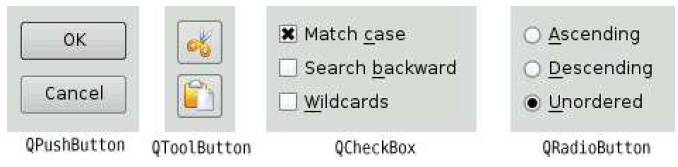
\includegraphics[width=9cm]{images/button_1.png}& 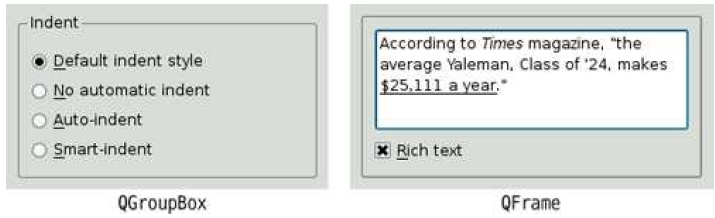
\includegraphics[width=9cm]{images/button_2.png}\\
	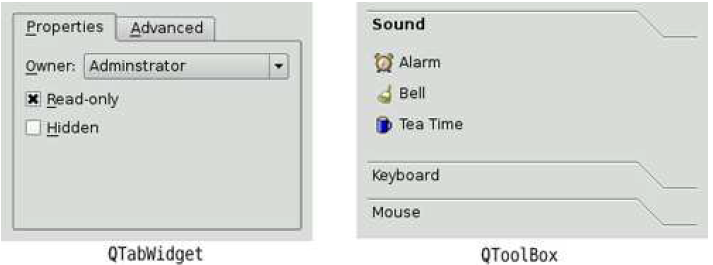
\includegraphics[width=9cm]{images/button_3.png}& 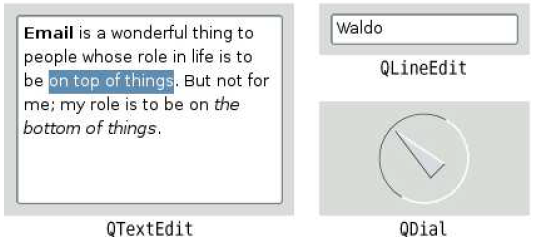
\includegraphics[width=9cm]{images/button_7.png}\\
	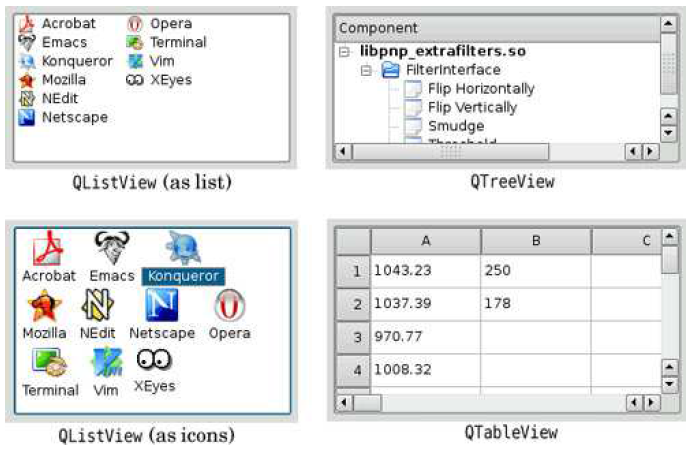
\includegraphics[width=9cm]{images/button_4.png}&
	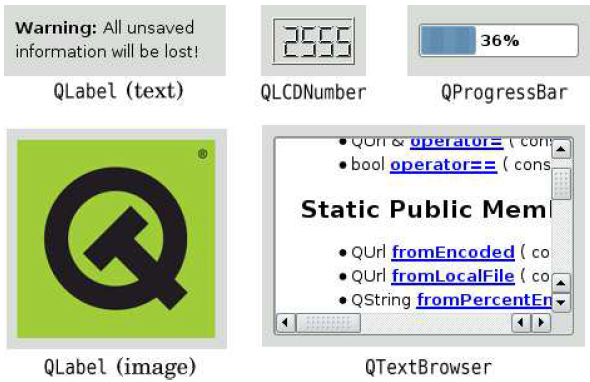
\includegraphics[width=9cm]{images/button_5.png}\\
	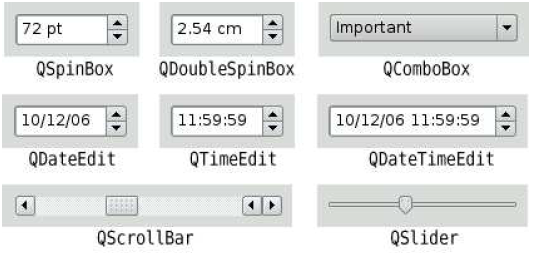
\includegraphics[width=9cm]{images/button_6.png}&
	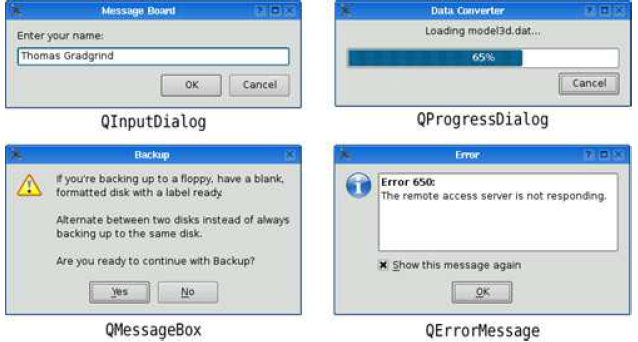
\includegraphics[width=9cm]{images/button_8.png}\\
\end{tabular}
\subsubsection{QBrush}
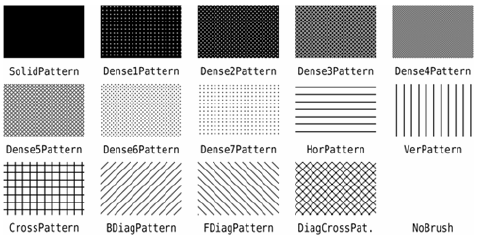
\includegraphics[width=9cm]{images/brush.png}

\subsubsection{QPainter draw-Methoden}
\begin{tabular}{c c}%TODO file doppelt
	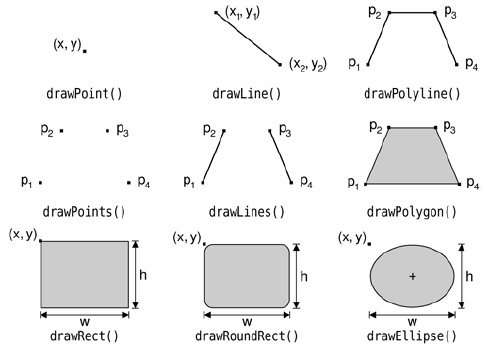
\includegraphics[width=9cm]{images/draw_1.png}& 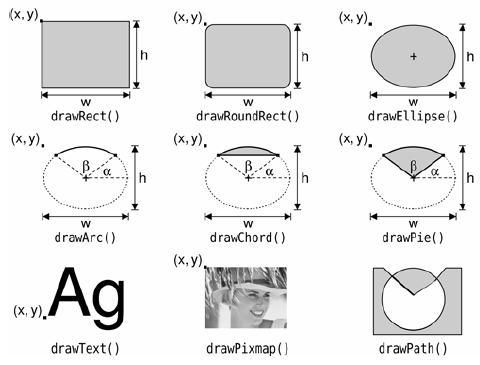
\includegraphics[width=9cm]{images/draw_2.png}\\
\end{tabular}
\subsubsection{QPen}
\begin{tabular}{c c}
	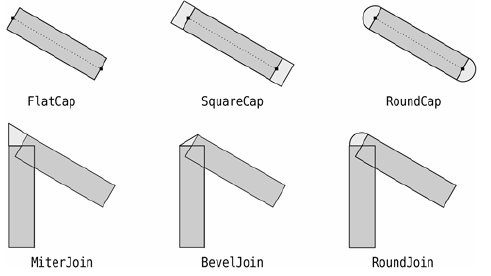
\includegraphics[width=9cm]{images/pen_1.png}& 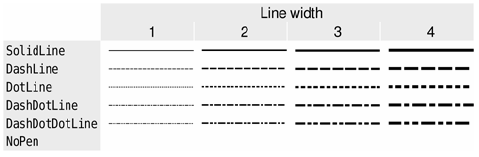
\includegraphics[width=9cm]{images/pen_2.png}\\
\end{tabular}

\subsubsection{SpezUeb}
\begin{longtable}{l l} %TODO: Layout
    \lstinputlisting[style=c++qt,linewidth=12cm]{source/Qt/SpezUeb1.cpp}&
    \includegraphics{images/qtSpezUeb1.jpg}
    \\
    \lstinputlisting[style=c++qt,linewidth=12cm]{source/Qt/SpezUeb2.cpp}&
    \includegraphics{images/qtSpezUeb2.jpg}
    \\
    \lstinputlisting[style=c++qt,linewidth=12cm]{source/Qt/SpezUeb3.cpp}&
    \includegraphics{images/qtSpezUeb3.jpg}
    \\
    \lstinputlisting[style=c++qt,linewidth=12cm]{source/Qt/GridLayout.cpp}&
    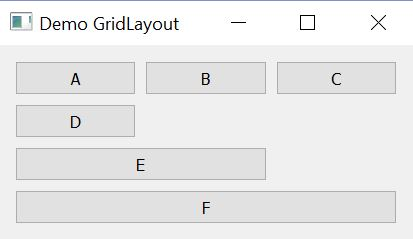
\includegraphics{images/GridLayout.jpg}    
\end{longtable}
%TODO JPG smaller
%\newpage 
%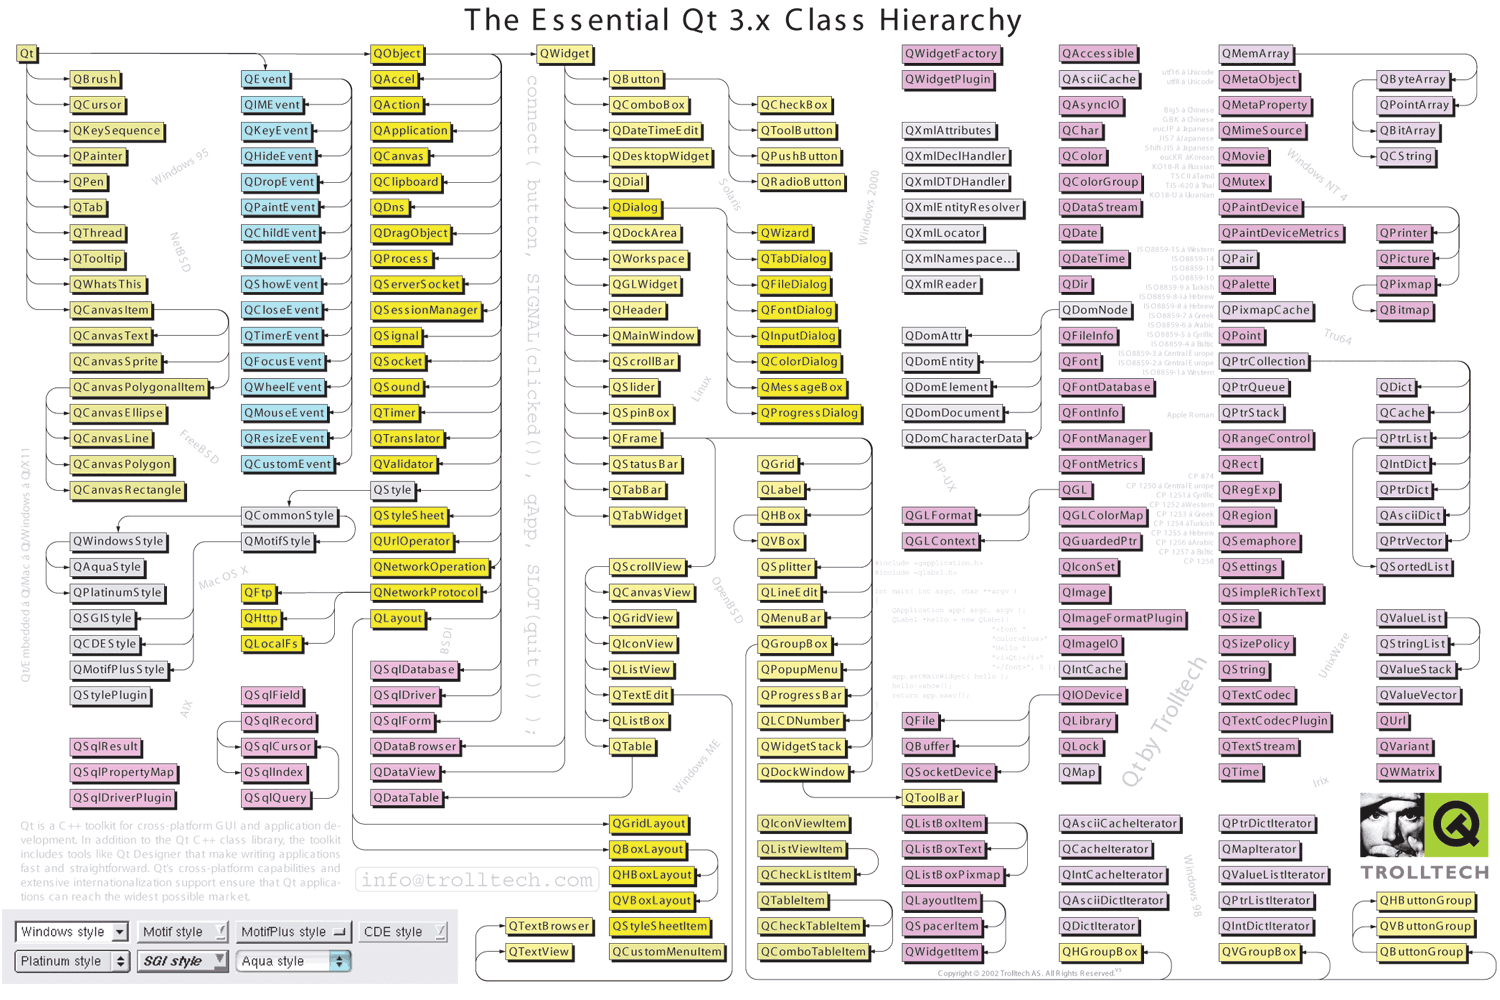
\includegraphics[angle=90,origin=c,width=\linewidth]{images/qt3classchart}
%\newpage
\subsubsection{Temperaturwidget}
\textbf{main.cpp}
\\
\lstinputlisting[style=c++qt]{source/Qt/main.cpp}
\textbf{temperaturwidget.h}
\\
\lstinputlisting[style=c++qt]{source/Qt/temperaturwidget.h}
\newpage
\textbf{temperaturwidget.cpp}
\lstinputlisting[style=c++qt]{source/Qt/temperaturwidget.cpp}